% Baccalauréat malgache, série C, 2015 : énoncé.
\TCDBacAttribution{C}{2015}
%%%%%%%%%%%%%%%%%%%%%%%%%%%%%%%%%%%%%%%%%%%%%%%%%%%%%%%%%%%%%%%%%%%%%%%%%%%%%%%%%%%%%%%%%%%%%%%%%%%%%%%%%%%%%%%%%%%%%%%%%%%%%%%%
\noindent \underline{\textsc{Exercice}} (4 points)% \newline
      \begin{description}
            \item[I.] \begin{enumerate}
                        \item R\'esoudre dans $\mathbb{Z}/7\mathbb{Z}$ l'\'equation : $\bar{6} x + \bar{2} = - \bar{3}$.
                        \item Soient $a$ et $b$ deux entiers relatifs premiers entre eux. \newline
                              D\'emontre que $A = 5 a + 3 b $ et $B = 8 a + 5 b $ sont aussi premier entre eux.
                        \item Soit $x \in \mathbb{N}$. \newline
                              Dans un syst\`eme de num\'eration \`a base 13, un entier naturel $M$ s'\'ecrit $ M = \bar{ \left( 25x3 \right) }_{_{13}}$.
                              \begin{enumerate}
                                    \item Justifier que : $M \equiv x+2 \quad [4]$.
                                    \item Pour quelles valeurs de $x$, $M$ est-il divisible par $4$\,?
                              \end{enumerate}
                  \end{enumerate}
            \item[II.] \begin{enumerate}
                        \item On lance une fois un d\'e t\'etra\'edrique parfait \`a quatre faces num\'erot\'ees 2, 3, 4 et 5 et
                              on s'interesse au num\'ero de la face cach\'ee. \newline
                              Calculer la probabilit\'e de chacun des \'ev\`enements suivants :
                              \begin{description}
                                    \item[A :] << La face cach\'ee porte le num\'ero inf\'erieur ou \'egal \`a 4 >>.
                                    \item[B :] << La somme des num\'eros des faces visibles est un nombre premier >>.
                              \end{description}
                        \item On lance maintenant $n$ fois de suite $(n \geq 2)$ le d\'e et on note 
                        $P_n$ la probabilit\'e de r\'ealiser au moins une fois l'\'ev\`enement
                         << la face cach\'ee porte un num\'ero inf\'erieur ou \'egal \`a 4 >> au cours de ces $n$ lancers.
                               \begin{enumerate}
                                     \item Calculer $P_3$.
                                     \item Donner le plus petit entier $n$ pour que $P_n \geq 0,99$.
                               \end{enumerate}
                  \end{enumerate}
      \end{description}
%
%%%%%%%%%%%%%%%%%%%%%%%%%%%%%%%%%%%%%%%%%%%%%%%%%%%%%%%%%%%%%%%%%%%%%%%%%%%%%%%%%%%%%%%%%%%%%%%%%%%%%%%%%%%%%%%%%%%%%%%%%%%%%%%%
\noindent \underline{\textsc{Probleme I}} (7 points) \newline
      $ABCDEF$ est un hexagone r\'egulier de centre $O$, de c\^ot\'e $a>0$
      dans un plan orient\'e $(\mathscr{P})$.
      Cet hexagone est direct donct : $(\overrightarrow{AB} ; \overrightarrow{AF}) = \frac{2\pi}{3} \quad [2\pi]$.
      On note par $I$ le milieu du segment $[AF]$.
      \begin{figure}[h!]
      \centering
            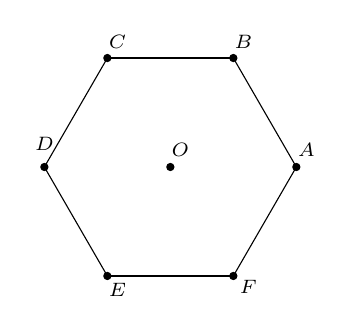
\begin{tikzpicture}[x=.8cm,y=.8cm]
            \draw (0,-1)-- (2,-1);
            \draw (2,-1)-- (3,0.73);
            \draw (3,0.73)-- (2,2.46);
            \draw (2,2.46)-- (0,2.46);
            \draw (0,2.46)-- (-1,0.73);
            \draw (-1,0.73)-- (0,-1);
            \begin{scriptsize}
            \fill [color=black] (0,-1) circle (1.5pt);
            \draw[color=black] (0.16,-1.22) node {$E$};
            \fill [color=black] (2,-1) circle (1.5pt);
            \draw[color=black] (2.24,-1.18) node {$F$};
            \fill [color=black] (3,0.73) circle (1.5pt);
            \draw[color=black] (3.16,1) node {$A$};
            \fill [color=black] (2,2.46) circle (1.5pt);
            \draw[color=black] (2.16,2.72) node {$B$};
            \fill [color=black] (0,2.46) circle (1.5pt);
            \draw[color=black] (0.16,2.72) node {$C$};
            \fill [color=black] (-1,0.73) circle (1.5pt);
            \draw[color=black] (-1,1.1) node {$D$};
            \fill [color=black] (1,0.73) circle (1.5pt);
            \draw[color=black] (1.16,1) node {$O$};
            \end{scriptsize}
            \end{tikzpicture}
      \end{figure}
      
      \noindent \underline{\textsc{Partie A}} \newline
      Soit $S$ un syst\`eme de trois points pond\'er\'es $(A;1);(B;-1);(D;1)$.
      \begin{enumerate}
            \item D\'eterminer et construire le barycentre $G$ de $S$.
            \item \begin{enumerate}
                        \item D\'eterminer et construire l'ensemble $(\Gamma)$ des 
                        points $M$ du plan $(\mathscr{P})$ qui v\'erifient 
                        $MA^2 - MB^2 + MD^2 = a^2$.
                        \item V\'erifier que $(\Gamma)$ passe par le centre de l'hexagone.
                  \end{enumerate}
      \end{enumerate}
      %
      \noindent \underline{\textsc{Partie B}} \newline
      Soit $R_O$ la rotation de centre $O$, d'angle $\frac{\pi}{3}$ 
      et $R_A$ la rotation de centre $A$, d'angle $\frac{2\pi}{3}$. \\
      Dans cette partie, on se propose de caract\'eriser la transformation 
      $f = R_A \circ R_O$, en utilisant deux m\'ethode diff\'erentes. \\
      %
            \noindent \underline{$\text{1}^\text{\`ere}$ m\'ethode} 
            \begin{enumerate}
                  \item Justifier que $f$ est une sym\'etrie centrale.
                  \item D\'eterminer l'image de $A$ par $f$, puis en d\'eduire le centre de $f$.
            \end{enumerate}
      %
            \noindent \underline{$\text{2}^\text{\`eme}$ m\'ethode} \\
            Le plan complexe est rapport\'e \`a un rep\`ere orthonorm\'e direct
            $(O ; \vec{u} , \vec{v})$ o\`u $\vec{u} = \vec{OA}$.
            \begin{enumerate}
                  \item Donner les affixes des points $A$, $F$ et $I$ le milieu de $[AF]$.
                  \item Ecrire les expressions complexes de $R_A$, $R_O$ et 
                        en d\'eduire celle de $f$.
                  \item D\'eterminer la nature et les \'el\'ements caract\'eristiques de $f$.
            \end{enumerate}
      %
      \noindent \underline{\textsc{Partie C}}% \newline
      \begin{enumerate}
            \item Soit l'application $g = R_O \circ R_O$.
                  \begin{enumerate}
                        \item D\'eterminer $g(A)$.
                        \item D\'eterminer l'\'ecriture complexe de $g$.
                        \item En d\'eduire les affixes des points $C$ et $E$.
                  \end{enumerate}
            \item Soit $\bar{S}$ la similitude plane indirecte qui transforme $O$ en $C$ et $A$ en $E$.
                  Donner l'\'ecriture complexe de $\bar{S}$.
                  En d\'eduire les \'el\'ements caract\'eristiques de $\bar{S}$.
      \end{enumerate}
%
%%%%%%%%%%%%%%%%%%%%%%%%%%%%%%%%%%%%%%%%%%%%%%%%%%%%%%%%%%%%%%%%%%%%%%%%%%%%%%%%%%%%%%%%%%%%%%%%%%%%%%%%%%%%%%%%%%%%%%%%%%%%%%%%
\noindent \underline{\textsc{Probleme II}} (9 points)% \newline
      \begin{center}
            \textbf{Les parties A et B sont ind\'ependantes.}
      \end{center}
      %
      \noindent \underline{\textsc{Partie A} : }% \newline
            On consid\`ere l'\'equation diff\'erentielle :
            \begin{equation*}
                  (E) : y'' + 2 y' - 3 y = P(x)
            \label{eq:diff2015}
            \end{equation*}
            o\`u $P$ est un polyn\^ome.
            \begin{enumerate}
                  \item Trouver le polyn\^ome $P$ pour que la fonction d\'efinie par $g$ d\'efinie par : 
                  $x \mapsto \expo{x} + x + 1$ soit une solution de $(E)$.
                  \item R\'esoudre l'\'equation diff\'erentielle 
                        $(E') : y'' + 2 y' - 3y = 0$.
                  \item Donner l'ensemble des solutions de $(E)$ que l'on note par $h$.
                        En d\'eduire la solution de $(E)$ qui satisfait aux conditions $h(O) = 1$ et $h'(O) = 5$.
            \end{enumerate}
      %
      \noindent \underline{\textsc{Partie B}} \newline
      Soit $f$ une fonction d\'efinie sur $[0 ; +\infty[$ par 
            \begin{displaymath}
                  f(x) = \begin{multiform}
                               \frac{x \ln x}{x+1}  \text{ si }  x>0        \\
                               0                    \text{ si }  x=0.
                         \end{multiform}
            \end{displaymath}
            On note par $(\mathscr{C})$ sa courbe repr\'esentative dans un rep\`ere orthonormal direct 
            $(O ; \vec{\imath} , \vec{\jmath})$ d'unit\'e 4~cm.
            %
            \begin{description}
                  \item[I-] \begin{enumerate}
                              \item Etudier la continuit\'e et la d\'erivabilit\'e de $f$ en $O$.
                              \item Soit $\varphi$ la fonction d\'efinie sur $]0 ; +\infty[$ par : 
                                    $\varphi (x) = - \ln x - x - 1$.
                                    \begin{enumerate}
                                          \item Etudier les variations de $\varphi$.
                                          \item Etablir que l'\'equation $\varphi(x) = 0$ admet une solution unique $\beta$ 
                                                et v\'erifier que $\beta \in\ ]0,27 \ ; \ 0,28[$. 
                                                (On ne demande pas de construire la courbe de $\varphi$).
                                                En d\'eduire le signe de $\varphi (x)$ suivant les valeurs de $x$ et 
                                                montrer que $f(\beta) = -\beta$.
                                    \end{enumerate}
                              \item Pour tout $x>0$, exprimer $f'(x)$ en fonction de $\varphi(x)$ 
                                    o\`u $f'$ est la d\'eriv\'ee de la fonction $f$.
                                    En d\'eduire les variations de $f$.
                              \item \begin{enumerate}
                                          \item Etudier la position relative de $(\mathscr{C})$ par rapport \`a la courbe 
                                                $(\Gamma)$ de la fonction $x\mapsto \ln x$ sur $]0 \ ; \ +\infty[$.
                                          \item Construire dans un rep\`ere les courbes $(\mathscr{C})$ et $(\Gamma)$. \par
                                          On donne $\ln (0,27) = -1,3$ ; $\ln (0,28) = -1,2$.
                                    \end{enumerate}
                        \end{enumerate}
                  \item[II-] On se propose d'\'etudier l'\'equation $f(x) = n$
                        o\`u $n$ est un entier naturel non-nul.
                        \begin{enumerate}
                              \item Montrer que, pour tout $n$, cette \'equation admet une solution unique not\'ee $\alpha_n$.
                              \item \begin{enumerate}
                                          \item \`Etablir que $f(\expo{n}) \leq n$. En d\'eduire que $\alpha_n \geq \expo{n}$.
                                          \item Prouver que la relation $f(\alpha_n) = n$ peut s'\'ecrire sous la forme 
                                                $\displaystyle{\ln \left( \frac{\alpha_n}{\expo{n}} \right) 
                                                      = \frac{n}{\alpha_n}} \qquad(1)$. \newline
                                                En d\'eduire, \` l'aide de $a)$, la limite de 
                                                $\frac{\alpha_n}{\expo{n}}$ lorsque $n$ tend vers l'infini.
                                    \end{enumerate}
                              \item On \'ecrit $\alpha_n$ sous la forme : 
                                    $\alpha_n = \expo{n} (1+\varepsilon_n)$ o\`u $\varepsilon_n \geq 0 \qquad (2)$.
                                    A l'aide de $(1)$, exprimer $(1+\varepsilon_n) \ln (1+\varepsilon_n)$ en fonction de $n$.
                              \item Soient $U$ et $V$ deux fonctions d\'efinies sur $[0 ; +\infty[$ par :
                                    \[
                                    U(t) = (1+t) \ln(1+t)   \text{ et }   V(t) = (1+t) \ln(1+t) - t - \frac{t^2}{2}.
                                    \]
                                    \begin{enumerate}
                                          \item Etudier les variations de $U$ et $V$, 
                                                puis en d\'eduire que pour tout $t \geq 0$, on a 
                                                $0 \leq (1+t) \ln(1+t) - t \leq \frac{t^2}{2}$.
                                          \item En utilisant $4)a)$ et $3)$, en d\'eduire que pour tout $n\geq 1$ : 
                                                $$\varepsilon \leq n \expo{-n} \leq \varepsilon_n + \frac{\varepsilon_n^2}{2}
                                                \text{, puis }
                                                0 \leq n \expo{-n} - \varepsilon_n \leq \frac{n^2}{2} \expo{-2n} \qquad(3)$$.
                                          \item A l'aide de $(2)$ et $(3)$, d\'eterminer 
                                                $\displaystyle{\lim_{n \rightarrow +\infty} (\expo{n} + n - \alpha_n )}$.
                                    \end{enumerate}
                        \end{enumerate}
            \end{description}
%%%%%%%%%%%%%%%%%%%%%%%%%%%%%%%%%%%%%%%%%%%%%%%%%%%%%%%%%%%%%%%%%%%%%%%%%%%%%%%%%%%%%%%%%%%%%%%%%%%%%%%%%%%%%%%%%%%%%%%%%%%%%%%%












































